\documentclass[conference]{IEEEtran}
\IEEEoverridecommandlockouts
\usepackage{cite}
\usepackage{amsmath,amssymb,amsfonts}
\usepackage{algorithmic}
\usepackage{graphicx}
\usepackage{textcomp}
\usepackage{xcolor}
\usepackage{hyperref}
\usepackage{makecell}
\usepackage{siunitx}
\def\BibTeX{{\rm B\kern-.05em{\sc i\kern-.025em b}\kern-.08em
    T\kern-.1667em\lower.7ex\hbox{E}\kern-.125emX}}
\begin{document}

%%%%%%%%%%%%%%%%%%%%%%%%%%%%%%%%%%%%%%%%%%%%%%%%%%%%%%%%%%%%%%%%%%%%%%%%%%%%%%%%%%
\title{
    HYDRA: High-Yield Data Reorganization \& Acceleration\\
    \large Midterm Report \\
}
%%%%%%%%%%%%%%%%%%%%%%%%%%%%%%%%%%%%%%%%%%%%
\author{
    \IEEEauthorblockN{
        Nafil Atiq\IEEEauthorrefmark{1},
        Ruohan Dong\IEEEauthorrefmark{1},
        Matthew Nutt\IEEEauthorrefmark{1},
        Giovanni Sirtori\IEEEauthorrefmark{1},
        Ben Wilson\IEEEauthorrefmark{1},
        Yulia Zhou\IEEEauthorrefmark{1}
}
%%%%%%%%%%%%%%%%%%%%%%%%%%%%%%%%%%%%%%%%%%%%
\IEEEauthorblockA{
    \IEEEauthorrefmark{1}%
    Department of Electrical \& Computer Engineering \\
    Rice University, Houston, Texas \\
    \{na115, rd100, mcn5, gs86, bjw8, yz305\}@rice.edu}
}
%%%%%%%%%%%%%%%%%%%%%%%%%%%%%%%%%%%%%%%%%%%%
\maketitle
%%%%%%%%%%%%%%%%%%%%%%%%%%%%%%%%%%%%%%%%%%%%%%%%%%%%%%%%%%%%%%%%%%%%%%%%%%%%%%%%%%
\begin{abstract}
    Data movement --- transposition, quantization, pooling, and
    non-contiguous gathers --- throttles AI inference on embedded RISC-V
    processors, consuming CPU cycles and polluting the L1 data cache.
    HYDRA (High-Yield Data Reorganization \& Acceleration) is a smart-DMA
    engine integrated as a second AHB-Lite master in the CORE-V Wally
    RV32GC SoC, with five modes: scatter-gather (A), corner-turning
    transposition (B), INT32-to-INT8 quantization (C), systolic INT8 GEMM
    (D), and streaming reduction (E). Modes~B, C, and~E are implemented,
    verified, and run end to end inside Wally from bare-metal C. A
    benchmarking methodology with explicit cache-state control shows that
    HYDRA streams one 32-bit word per cycle after a fixed cost
    (98.25\% of peak AHB bandwidth); Mode~B is 4.41$\times$ faster than
    optimized software when data fits in the 16~KiB D-cache and
    5.42$\times$ at 8192 words, and Mode~E max-pooling reaches
    3.78$\times$. The team also synthesized HYDRA on ASAP7, began FPGA
    emulation, and built UVM environments for HYDRA and for a RISC-V data
    cache.
\end{abstract}
%%%%%%%%%%%%%%%%%%%%%%%%%%%%%%%%%%%%%%%%%%%%%%%%%%%%%%%%%%%%%%%%%%%%%%%%%%%%%%%%%%
\begin{IEEEkeywords}
    RISC-V, DMA, hardware acceleration, AHB-Lite, SystemVerilog, UVM,
    quantization, pooling, systolic array, performance characterization
\end{IEEEkeywords}
%%%%%%%%%%%%%%%%%%%%%%%%%%%%%%%%%%%%%%%%%%%%%%%%%%%%%%%%%%%%%%%%%%%%%%%%%%%%%%%%%%
\section{Introduction}
    Processor performance has long outpaced memory
    bandwidth~\cite{wulf1995}, and AI inference widens the gap: model size
    and compute have grown far faster than memory
    bandwidth~\cite{gholami2024}. Inference also spends much of its time
    only reorganizing data (layout conversion, quantization, pooling,
    gathers), which on an embedded core runs as load/store loops that
    stall the pipeline and evict useful cache lines. Conventional DMA
    engines such as the TI EDMA~\cite{ti_edma} move contiguous blocks but
    cannot transform data in flight, while ML accelerators are large and
    tied to narrow operator sets. HYDRA sits between the two: a
    programmable DMA engine that transforms data while it moves. It
    integrates into the CORE-V Wally SoC~\cite{harris2025wally} as a second
    AHB-Lite master, reusing Wally's verified core, caches, and bus.
 
    This report covers HYDRA's RTL and SoC integration (Modes~B, C,
    and~E), its benchmarking methodology and results, standalone ASAP7
    synthesis, FPGA emulation, and UVM verification of HYDRA and of a
    RISC-V data cache.
%%%%%%%%%%%%%%%%%%%%%%%%%%%%%%%%%%%%%%%%%%%%%%%%%%%%%%%%%%%%%%%%%%%%%%%%%%%%%%%%%%
\section{Methods}
%%%%%%%%%%%%%%%%%%%%%%%%%%%%%%%%%%%%%%%%%%%%
    \subsection{RTL Design and SoC Integration}
        HYDRA is implemented as a second AHB-Lite~\cite{amba_ahb} bus master
        in the Wally SoC, peer to the CPU's External Bus Unit, following the
        modular front-end / mid-end / back-end DMA decomposition of Benz
        et al.~\cite{benz2024}.
        \texttt{hydra\_mmr.sv} implements the AHB slave register file (front-end), 
        exposing CTRL, SRC, DST, LEN, and STATUS registers to the CPU.
        \texttt{hydra\_transform.sv} contains the address generation unit and 
        the transformation datapath (mid-end), together with the AHB master 
        state machine that issues burst transactions on the data plane (back-end). 
        \texttt{hydra\_arbiter.sv} mediates bus contention between HYDRA and 
        the CPU through a Moore FSM with a registered grant output, breaking 
        any combinational path from \texttt{HBUSREQ} to \texttt{HADDR}. 
        \texttt{hydra\_scratchpad.sv} is a 32~KB ($8192 \times 32$-bit)
        single-port memory, the smallest size that holds the outputs of the
        benchmark workloads. Two requesters share its one port: an AHB-Lite
        slave interface for CPU reads and a private sideband write port for
        HYDRA. Keeping HYDRA's writes off the AHB fabric is essential ---
        routing them through the bus would serialize them with HYDRA's own
        read transactions, eliminating the fill/drain overlap that Mode~B's
        ping-pong design relies on. HYDRA's write always takes the port. If a
        CPU read collides with it, the scratchpad captures the read address,
        holds \texttt{HREADYOUT} low while HYDRA writes, and serves the held read
        on the next free cycle, so the CPU receives post-write data and
        nothing is corrupted. Because software reads the scratchpad only
        after HYDRA reports completion, collisions are rare, and a single
        port costs half the memory ports of the earlier dual-port design. The
        full topology is shown in Fig.~\ref{fig:hydra-block}.

        \begin{figure}[t]
        \centering
        \fbox{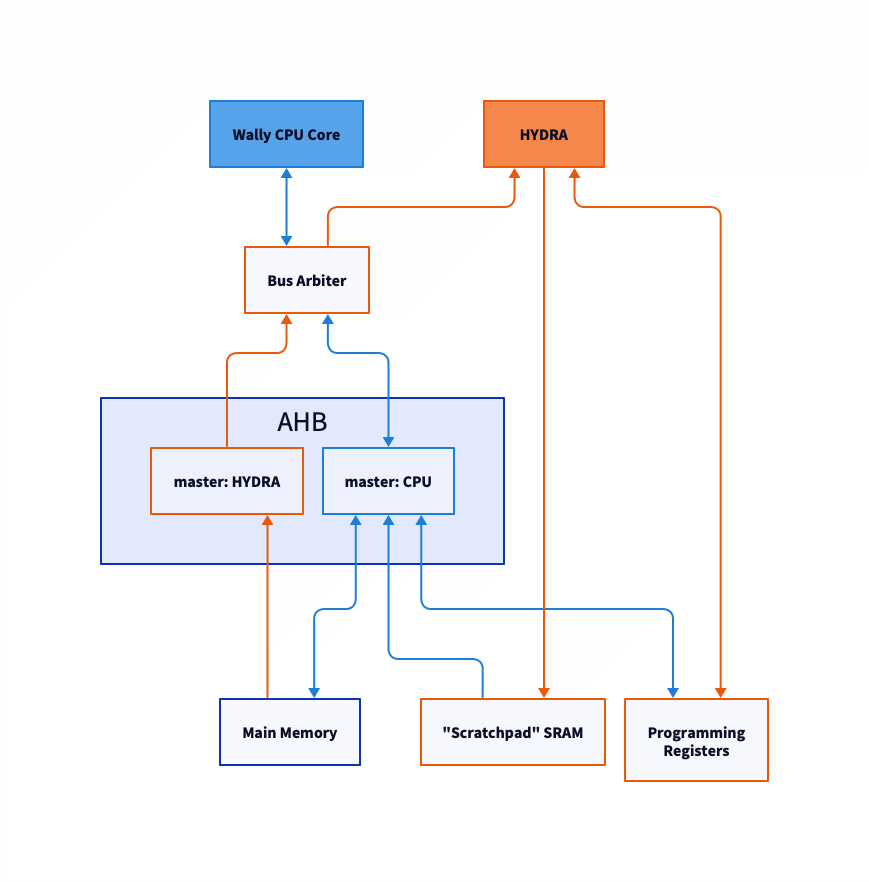
\includegraphics[width=0.6\linewidth]{figures/HYDRA_diag.png}}
        \caption{Full system block diagram.}
        \label{fig:hydra-block}
        \end{figure}
        
        Mode~B (Corner-Turning) partitions the source matrix into $8 \times 16$ 
        blocks of 32-bit words, exactly matching one Wally cache line per row, following the block corner-turning method of Ma et al.~\cite{ma2019}. 
        Two ping-pong SRAM buffers operate concurrently: one drains column-major 
        to the scratchpad while the other fills row-major from main RAM. An 
        early-drain optimization further reduces per-block latency by exploiting 
        the row-major-fill / column-major-drain index skew. Drain can begin on 
        the same buffer still being filled provided the fill counter leads the 
        drain counter by at least $(N-1)(M-1) = 105$ beats, saving 22 of the 
        128 cycles otherwise spent waiting for the first buffer to complete 
        before standard ping-pong overlap takes over.
        
        Mode~C implements a fully combinational rounding-and-saturation
        pipeline (\texttt{quant\_fn} in \texttt{hydra\_pkg.sv}) that converts
        INT32 inputs to INT8 outputs, the integer format standard for
        efficient inference~\cite{jacob2018}, and packs four results into
        each 32-bit scratchpad word. HYDRA still reads one 32-bit word per
        cycle, but the output footprint, and therefore the data a consumer
        later reads from the scratchpad, shrinks by 4$\times$, per
        Equation~\ref{eq:bw}. Scale shift, signed/unsigned output, and
        round-half-up rounding are configurable at runtime through MMR
        fields, so the same hardware serves signed (e.g., audio) and
        unsigned (e.g., image) data.
        
        \begin{equation}
        B_{\text{eff}} = B_{\text{raw}} \times \frac{W_{\text{src}}}{W_{\text{dst}}}
        \label{eq:bw}
        \end{equation}

        Mode~E (Reduction) splits the source stream into non-overlapping
        windows of \texttt{POOL\_SIZE} 32-bit words (a compile-time power of
        two, default 4) and reduces each to one word using a runtime-selected
        operator: signed sum, maximum, minimum, or average. \texttt{reduce\_fn}
        in \texttt{hydra\_pkg.sv} folds each \texttt{HRDATA} beat into a single
        accumulator as it arrives and writes the result to the scratchpad on
        the window's last beat. Mode~E therefore streams at one word per beat
        with no buffering or flush phase, and
        $W_{\text{src}}/W_{\text{dst}} = $ \texttt{POOL\_SIZE} in
        Equation~\ref{eq:bw}.

        The MMR was extended for Mode~E and a safer CPU handshake. CTRL gains
        a REDUCE\_OP field and a MODE field widened to three bits, and STATUS
        gains a BUSY bit. While BUSY is set, MMR writes are ignored, and a new
        START clears DONE and ERROR. Requests whose output would overrun the
        scratchpad are rejected to the ERROR state.

        Coherency is handled differently on the two sides of a transfer
        (Table~\ref{tab:memmap}). On the destination side it holds by
        construction: HYDRA writes only to the non-cacheable scratchpad
        (\texttt{0x2001\_0000}), so no cached line ever goes stale. The
        source side requires software cooperation: HYDRA reads main RAM
        directly, while Wally's L1 data cache is write-back, so any dirty
        source lines must be written back before launch. The driver does
        this with the Zicbom~\cite{riscv_cmo} \texttt{cbo.clean} (or
        \texttt{cbo.flush}) instruction over the source range. The MMR
        slave is zero-wait-state, with \texttt{HREADYOUT} permanently
        asserted; the scratchpad inserts wait states only when a CPU read
        collides with a HYDRA write. Wally is integrated as a Git
        submodule with patches applied through a reproducible script
        workflow, keeping the HYDRA repository lightweight and
        version-agnostic across Wally upstream changes.
        
        \begin{table}[t]
        \caption{HYDRA memory map (additions to Wally)}
        \label{tab:memmap}
        \centering
        \begin{tabular}{llll}
        \hline
        \textbf{Region} & \textbf{Base Address} & \textbf{Size} & \textbf{Attribute} \\
        \hline
            HYDRA MMR        & \texttt{0x2000\_0000} & 4 KB   & Non-cacheable \\
            Scratchpad SRAM  & \texttt{0x2001\_0000} & 32 KB  & Non-cacheable \\
            Main RAM         & \texttt{0x8000\_0000} & 128 MB & Cached (I\$/D\$) \\
        \hline
        \end{tabular}
        \end{table}
%%%%%%%%%%%%%%%%%%%%%%%%%%%%%%%%%%%%%%%%%%%%
    \subsection{Benchmarking Methodology}
        HYDRA is benchmarked on the RV32GC Wally SoC in Questa with a
        bare-metal C harness. For each transfer size, the harness times
        two kernels with the \texttt{mcycle} and \texttt{minstret}
        counters: the HYDRA driver (programming the MMR, then polling
        STATUS) and an optimized software implementation of the same
        transform. The timed window covers the full offload, including
        MMR programming, the transfer, and completion detection. The
        software baseline is compiled with \texttt{-O3 -funroll-loops},
        uses \texttt{restrict} pointers, and writes its output sequentially
        into cacheable RAM, its natural destination.

        Cache state is set explicitly before every timed run. In the
        headline regime (WICD: warm I-cache, cold D-cache), one
        discarded warm-up run of each kernel trains the I-cache and branch
        predictor, and \texttt{cbo.flush} then writes back and invalidates
        the source and destination lines. Two secondary regimes bracket
        it: CICD (cold I-cache, cold D-cache) adds \texttt{fence.i}, which
        on Wally invalidates the I-cache but only writes back the
        D-cache, and WIWD (warm I-cache, warm D-cache) uses
        \texttt{cbo.clean}, which writes dirty lines back to RAM for
        HYDRA's benefit while keeping them resident for the software.

        Both timed kernels are marked \texttt{noipa}, so the compiler
        cannot inline or specialize them per transfer size, and every
        counter read carries a \texttt{"memory"} clobber so no load or
        store can move across a timestamp. A hardware fence is unnecessary
        because an ordinary \texttt{FENCE} is a no-op on Wally's in-order
        core. Every output is checked against a seeded golden pattern,
        pre-filled with a poison value, outside the timed window. To
        explain software behavior beyond cache capacity, we also built a
        Python model of Wally's 16~KiB, 4-way, pseudo-LRU, write-back data
        cache that predicts misses and dirty writebacks per block.
%%%%%%%%%%%%%%%%%%%%%%%%%%%%%%%%%%%%%%%%%%%%
    \subsection{FPGA Implementation}
        Running Wally with HYDRA on an FPGA provides hardware validation and
        FPGA-level power, timing, and resource figures. We use AMD Vivado to
        synthesize and implement the design, with a constraints file setting
        the target clock and I/O, and Tcl scripts that automate the flow
        without the GUI.
        
%%%%%%%%%%%%%%%%%%%%%%%%%%%%%%%%%%%%%%%%%%%%
    \subsection{ASIC Implementation}
        Simulated speedups matter only if HYDRA's area, power, and frequency
        costs are acceptable, so we compare the PPA of Wally with and without
        HYDRA. The flow targets ASAP7, a predictive 7\,nm PDK~\cite{asap7pdk}
        with no license or NDA requirements, using its 7.5-track cell
        library~\cite{asap7cell} and 6-track SRAM macros~\cite{asap7sram},
        and Cadence Genus and Innovus. Synthesis uses a constraints file
        (clock and I/O delays), an MMMC file for the PVT corners, and a main
        script; the RTL was modified to remove unsynthesizable constructs and
        to instantiate SRAM macros in place of explicit registers.
        
%%%%%%%%%%%%%%%%%%%%%%%%%%%%%%%%%%%%%%%%%%%%
    \subsection{UVM Verification for HYDRA}
        Two independent UVM environments were developed for unit-level verification of the HYDRA memory-mapped registers (MMR) and the Mode C transform. In the MMR environment, a CPU-side AHB agent writes configuration registers and reads them back. A monitor observes the bus transactions, while a scoreboard checks readback values, register independence, and reset behavior.

        The Mode C environment tests the transform directly, without programming it through the MMR. A control sequence provides the configuration and start signal. Before each test, input words are prepared in a RAM model; a RAM responder returns those values when the DUT issues read requests. Monitors capture the control settings, RAM reads, and scratchpad writes. The scoreboard checks read addresses and counts, output data, and how four output bytes are packed into each scratchpad word. Directed tests exercise arithmetic settings, multiple output words, wait states, arbitration, invalid length, and back-to-back operations.
        
%%%%%%%%%%%%%%%%%%%%%%%%%%%%%%%%%%%%%%%%%%%%
    \subsection{Data Cache Verification Framework}
        A layered UVM testbench (test, environment, CPU agent with
        sequencer, driver, and monitor, and scoreboard) verifies a 2~KB
        direct-mapped, write-through, no-write-allocate data cache with
        32-byte lines. The scoreboard's reference model tracks expected
        memory and cache state and checks every transaction. Stimulus is
        constrained-random: each transaction picks a read or write and an
        address from four weighted patterns (repeat address for hits, same
        line for word offsets, same index with a new tag for conflict
        misses, and new address for compulsory misses).
%%%%%%%%%%%%%%%%%%%%%%%%%%%%%%%%%%%%%%%%%%%%
     
%%%%%%%%%%%%%%%%%%%%%%%%%%%%%%%%%%%%%%%%%%%%%%%%%%%%%%%%%%%%%%%%%%%%%%%%%%%%%%%%%%
\section{Results}
%%%%%%%%%%%%%%%%%%%%%%%%%%%%%%%%%%%%%%%%%%%%
    \subsection{RTL Design}
        The full HYDRA RTL hierarchy is implemented in synthesizable 
        SystemVerilog: \texttt{hydra\_pkg.sv} (shared types and the 
        \texttt{quant\_fn} and \texttt{reduce\_fn} quantization and pooling functions), \texttt{hydra\_top.sv}, 
        \texttt{hydra\_mmr.sv}, \texttt{hydra\_arbiter.sv}, 
        \texttt{hydra\_scratchpad.sv}, and \texttt{hydra\_transform.sv}. A 
        self-checking testbench exercises fifteen directed test cases covering 
        Mode~B (single- and multi-block transfers, HREADY wait-state injection, 
        HRESP error injection, and invalid-length ERROR\_HALT), Mode~C 
        (signed and unsigned outputs, varying scale shifts, and saturation
        corners), and Mode~E (sum across multiple bursts,
        signed max and min with negative inputs, average, and rejection of a
        misaligned length). All three modes pass functional verification in
        Questa (15 tests, 0 errors): the AHB
        master FSM issues bursts with correct NONSEQ/SEQ pipelining, 
        the ping-pong buffer overlaps fill and drain as designed, and the 
        combinational quantization path produces bit-exact results against a 
        golden model. With the integration patches to Wally's
        \texttt{wallypipelinedsoc.sv}, \texttt{uncore.sv},
        \texttt{adrdecs.sv}, \texttt{cvw.sv}, \texttt{parameter-defs.vh}, 
        \texttt{plic\_apb.sv}, \texttt{pmachecker.sv} and \texttt{config.vh}
        applied, HYDRA runs end to end inside the Wally SoC, driven from 
        bare-metal C, and every benchmark run in Section~\ref{sec:perf} 
        produced outputs that matched the golden model.
%%%%%%%%%%%%%%%%%%%%%%%%%%%%%%%%%%%%%%%%%%%%
%%%%%%%%%%%%%%%%%%%%%%%%%%%%%%%%%%%%%%%%%%%%
    \subsection{Performance Characterization}
    \label{sec:perf}
        \textit{Mode~B.} Mode~B was characterized over 64 transfer sizes
        ($L = 128$ to 8192 words, in 128-word blocks), three cache regimes,
        and four compiler optimization levels. HYDRA's cycle count fits
        $T_{\text{HYDRA}} \approx 146 + 1.00\,L$ (RMSE $\approx$ 2 cycles)
        and is identical in every cache regime: once launched, HYDRA
        streams one 32-bit word per cycle, the full AHB bandwidth. Bus
        efficiency, $L/(146+L)$, therefore rises from 46.38\% at
        $L = 128$ to 98.25\% at $L = 8192$.

        \begin{figure}[t]
        \centering
        \fbox{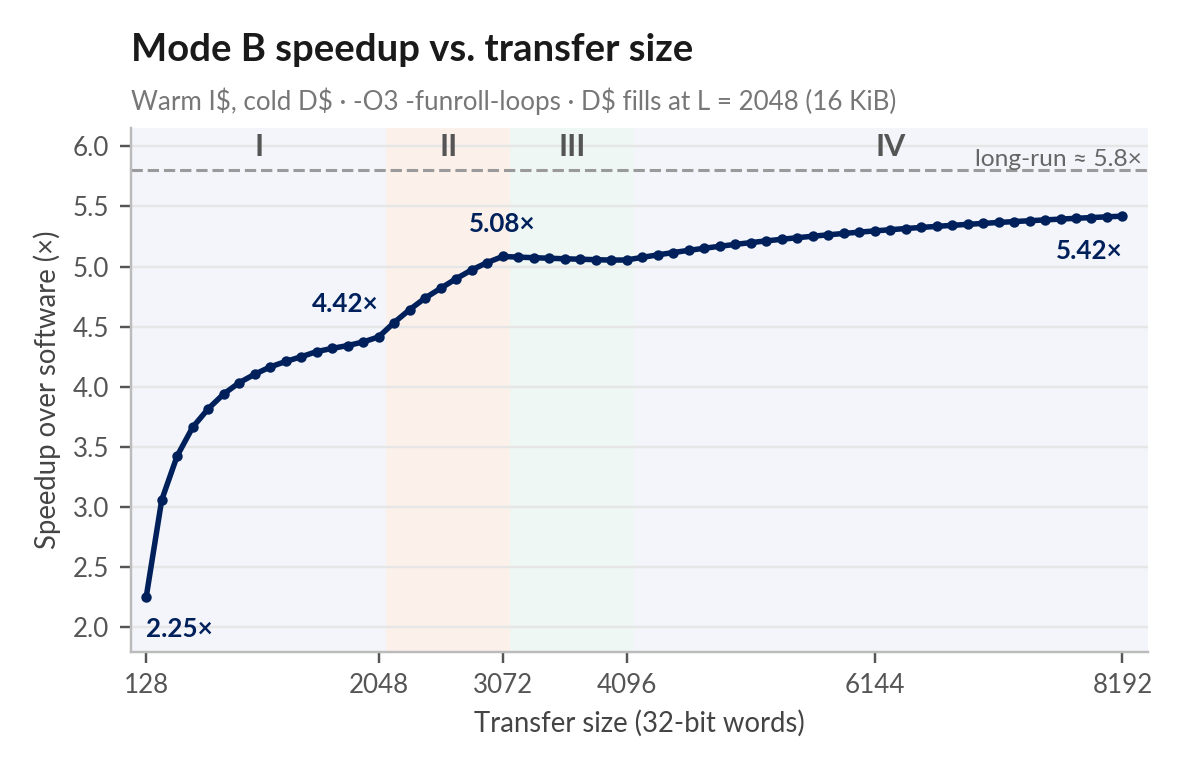
\includegraphics[width=0.8\linewidth]{figures/hydra_modeB_speedup.png}}
        \caption{Mode~B speedup over software (WICD, \texttt{-O3
        -funroll-loops}). Regions I--IV are dirty-writeback phases of the
        software kernel after the D-cache fills at $L = 2048$.}
        \label{fig:modeB-speedup}
        \end{figure}

        In the headline regime (Fig.~\ref{fig:modeB-speedup}), speedup grows
        from 2.25$\times$ at 128 words to 4.41$\times$ at 2048 words, where
        source and destination together fill the 16~KiB D-cache. Up to that
        point the software kernel costs 4.72 cycles per element, so the
        speedup approaches 4.7$\times$ as HYDRA's fixed cost is amortized.
        Beyond capacity, the software kernel also pays dirty-line
        writebacks of about 18 cycles each. Their count per block depends
        on how the source and destination streams alias in the pseudo-LRU
        cache, producing the four regions in the figure, and our cache
        model reproduces the measured per-block cost of every region
        within 2\%. Because each block dirties eight lines, every buffer
        layout converges to eight writebacks per block (5.80 cycles per
        element), so the speedup reaches 5.42$\times$ at 8192 words and
        tends toward 5.8$\times$. HYDRA's cost is unaffected throughout.

        \begin{table}[h]
        \caption{Mode~B speedup over software}
        \label{tab:modeB}
        \centering
        \begin{tabular}{llcc}
        \hline
        \textbf{Sweep} & \textbf{Configuration} & $L = 128$ & $L = 2048$ \\
        \hline
            Cache regime  & CICD                            & 2.65$\times$ & 4.45$\times$ \\
            \makecell[l]{(\texttt{-O3 \textbackslash}\\
            \texttt{-funroll-loops})}                       & \textbf{WICD (headline)} &                                                             \textbf{2.25$\times$} &                                                                \textbf{4.41$\times$} \\
                          & WIWD                            & 1.21$\times$ & 2.34$\times$ \\
        \hline
            Compiler      & \texttt{-O1}                    & 4.35$\times$ & 8.52$\times$ \\
            (WICD)        & \texttt{-O2}                    & 3.89$\times$ & 7.68$\times$ \\
                          & \texttt{-O3}                    & 2.26$\times$ & 4.41$\times$ \\
                          & \makecell[l]{\texttt{-O3 \textbackslash} 
                            \\\texttt{-funroll-loops}}     
                                                            & \textbf{2.25$\times$} & \textbf{4.41$\times$} \\
        \hline
        \end{tabular}
        \end{table}

        Table~\ref{tab:modeB} shows how sensitive the result is to the
        baseline. A cold I-cache adds about 125--200 cycles to the software
        kernel but at most about 20 to HYDRA's small driver, so CICD gives
        the largest speedup at small sizes. WIWD is the software's best
        case, with the source already cached, and still yields at least
        1.21$\times$: HYDRA is faster at every size in every regime. Going
        to \texttt{-O3} is the largest single improvement in the software
        kernel, while adding \texttt{-funroll-loops} changes the speedup by
        at most 0.01$\times$, consistent with a memory-bound kernel. All
        headline figures use the strongest baseline.

        \textit{Mode~C.} Mode~C reads one 32-bit word per cycle, like Mode~B,
        but writes one byte per input word, packing four INT8 results into
        each scratchpad word. The output footprint, and with it the data a
        consumer later reads from the scratchpad, shrinks by 4$\times$, a
        4$\times$ gain in effective bandwidth per Equation~\ref{eq:bw}.

        \textit{Mode~E.} Mode~E was benchmarked as a signed max-pool with the
        same methodology (warm I-cache, cold D-cache, \texttt{-O3
        -funroll-loops}).

        \begin{figure}[t]
        \centering
        \fbox{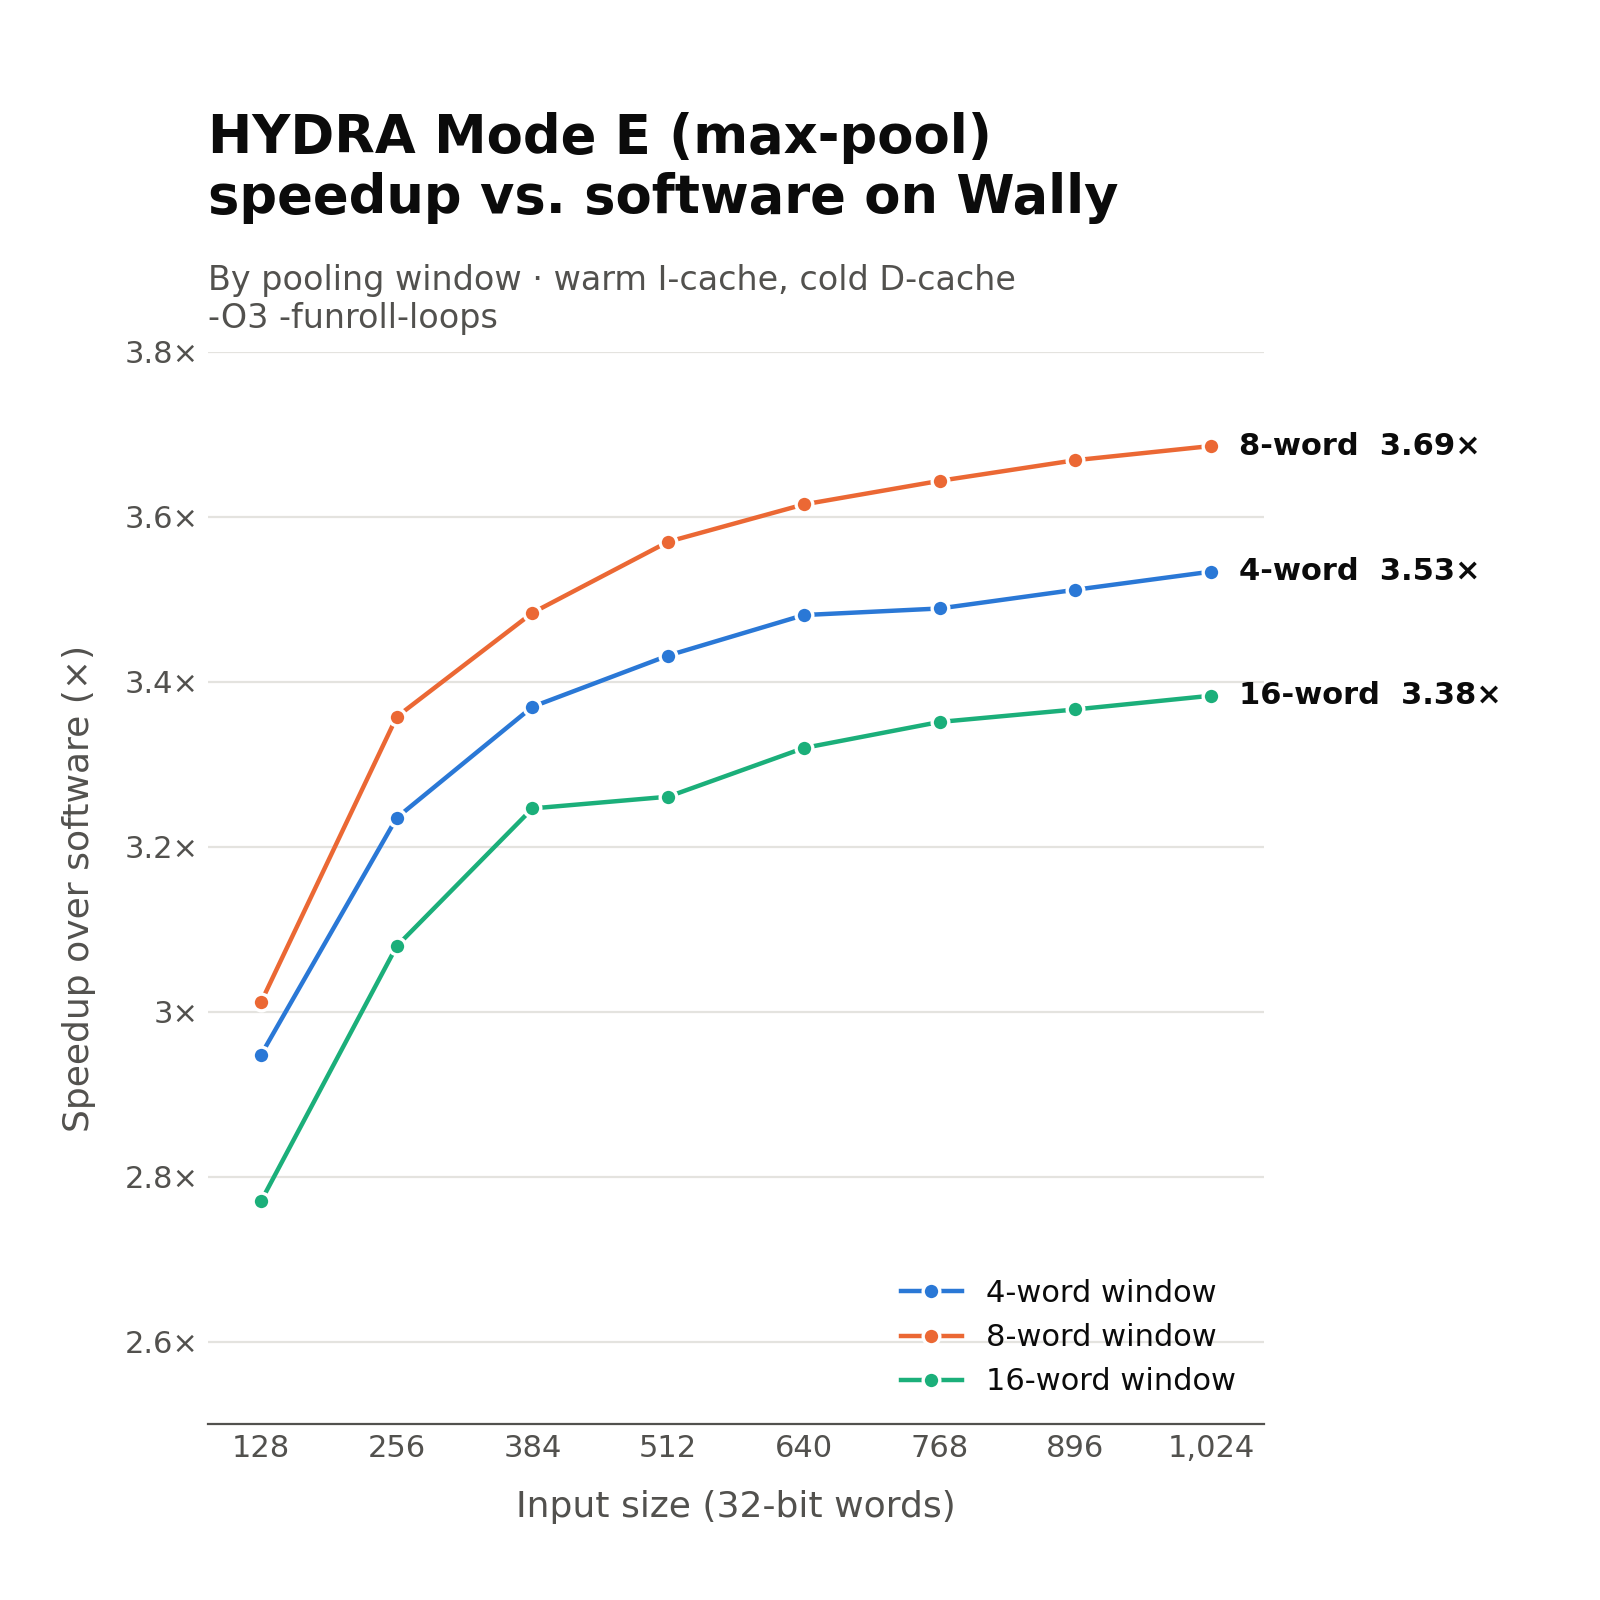
\includegraphics[width=0.7\linewidth]{figures/hydra_modeE_pool_sweep_128-1024_square.png}}
        \caption{Mode~E max-pool speedup over software on Wally for 4-, 8-,
        and 16-word windows.}
        \label{fig:modeE-speedup}
        \end{figure}

        As Fig.~\ref{fig:modeE-speedup} shows, speedup grows from
        2.8--3.0$\times$ at 128 words to 3.4--3.7$\times$ at 1024 words,
        reaching 3.78$\times$ at 8192 words (a 4-word window, filling 8~KB of
        the scratchpad). HYDRA's cost is about one cycle per input word plus
        a fixed setup and polling overhead of roughly 45 cycles, using 21
        instructions at every size, so speedup rises as that overhead is
        amortized. HYDRA's time is nearly independent of window size; the
        spread between windows comes from how well the compiler unrolls the
        software loop, which is best for 8-word windows.
%%%%%%%%%%%%%%%%%%%%%%%%%%%%%%%%%%%%%%%%%%%%
    \subsection{FPGA Implementation}
        The first part of the FPGA Emulation was to synthesize and implement HYDRA as a standalone module. HYDRA was successfully synthesized and implemented using Vivado's GUI. Following the synthesis of HYDRA, PPA results were available. Along with that, a constraints file for HYDRA alone was created to be able to use different clock speeds. Lastly for HYDRA, a tcl file was made that automatically synthesized and implemented HYDRA and outputted report files. This program could then be run through C by a System command to use Vivado's batch functionality.
%%%%%%%%%%%%%%%%%%%%%%%%%%%%%%%%%%%%%%%%%%%%
    \subsection{ASIC Implementation}
        The first goal for the ASIC implementation was synthesis of the HYDRA system as a standalone module. Following the installation of ASAP7 on the Rice CLEAR servers, the development of the necessary scripts, and modifications to HYDRA RTL, synthesis with Genus was successful, and generated an output netlist for use in place-and-route.

        In addition, Genus provided several reports on post-synthesis PPA figures. As a standalone module, HYDRA successfully meets timing under a \SI{500}{\mega\hertz} clock, takes up \SI{116586}{\micro\meter\squared} (estimated) area, and consumes \SI{11.7}{\milli\watt} of power.
%%%%%%%%%%%%%%%%%%%%%%%%%%%%%%%%%%%%%%%%%%%%
    \subsection{UVM Verification for HYDRA}
        The MMR tests passed checks for register readback, independence, data patterns, and reset values. The completed Mode C directed tests also passed in their final runs. The basic test showed why checking only the final output is insufficient: although four input words produced the correct packed scratchpad value, the DUT read the first RAM address twice and later requested an address outside the prepared input range.

        The issue was traced to Mode C address generation. After the RTL was changed to advance and count accepted RAM reads, the basic test completed with four reads and one correct scratchpad write. An eight-input regression produced eight reads and two correctly packed output words. Other tests covered wait states, arbitration, and back-to-back operations. The invalid-length test confirmed that length=9 was rejected without RAM reads or scratchpad writes. In the combined-arithmetic test, four operations completed with 32 reads, eight writes, and no UVM errors.
%%%%%%%%%%%%%%%%%%%%%%%%%%%%%%%%%%%%%%%%%%%%
    \subsection{Data Cache Verification Results}
        This semester, the constrained-random stimulus randomizes both the operation type and the address of each transaction, choosing from four address patterns: same address, same cache line, same index, and new address.

        Two bugs in the memory interface were identified and fixed. In the first, the last word of a refilled line read back as zero because the memory data arrived one cycle after the burst ended; a new state now waits one cycle to capture it. In the second, back-to-back misses returned stale data because an extra burst started after each miss; the fix ignores the request in the cycle that ready is returned. After both fixes, all seeds passed without scoreboard mismatches.
%%%%%%%%%%%%%%%%%%%%%%%%%%%%%%%%%%%%%%%%%%%%
    
%%%%%%%%%%%%%%%%%%%%%%%%%%%%%%%%%%%%%%%%%%%%%%%%%%%%%%%%%%%%%%%%%%%%%%%%%%%%%%%%%%
\section{Discussion}
%%%%%%%%%%%%%%%%%%%%%%%%%%%%%%%%%%%%%%%%%%%%
%%%%%%%%%%%%%%%%%%%%%%%%%%%%%%%%%%%%%%%%%%%%
    \subsection{HYDRA RTL and Integration}
        Benchmarking clarified where HYDRA's remaining cost lies. Mode~E's
        fixed overhead is about 45 cycles, whereas Mode~B's is 146. The
        difference is consistent with Mode~B's corner-turning drain tail:
        with early drain, draining a block can begin only once the fill
        leads by 105 beats, so the final block finishes draining about 105
        cycles after its last read. Most of Mode~B's fixed cost is
        therefore inherent to transposing in blocks rather than launch
        overhead. Benchmarking also showed that source-side coherency must
        be explicit: the driver must clean dirty source lines before every
        launch, so a cache-maintenance helper will be part of HYDRA's
        software interface.

        Work this semester continues on two fronts. First, Mode~A
        (scatter-gather) adds descriptor fetch, where each descriptor holds
        a source address, a length, and a pointer to the next one, on top
        of the AHB master FSM already validated for Modes~B, C, and~E; it
        targets at least 90\% bus efficiency on contiguous runs of 256 words
        or more. Second, Mode~D adds a 4$\times$4 weight-stationary systolic
        array~\cite{kung1982, jouppi2017} for INT8 GEMM with 32-bit
        accumulators. To feed it from data already in the scratchpad,
        a mode-selectable source field in the MMR will let any transform
        read either from main memory over AHB or directly from the
        scratchpad, avoiding a second trip through main memory. The benchmarking 
        harness will be reused for Modes~A and D, so every mode is reported with
        the same methodology.
%%%%%%%%%%%%%%%%%%%%%%%%%%%%%%%%%%%%%%%%%%%%
    \subsection{ASIC Implementation}
        With the proof-of-concept of standalone synthesis, work continues toward synthesizing the full Wally SoC. Besides the usual elimination of unsynthesizable RTL, Wally's design is offering additional challenges: The largest SRAM macro offered by the ASAP7 PDK is \SI{10}{\kilo B}, whereas the SoC demands multi-megabyte storage. The SoC also expects byte-wise write capability, while the macros are only word-wise write capable. Mitigating these discrepancies may require extensive RTL modifications, especially if SRAM adaptations will require stall cycles to complete byte-wise writes.

        As insufficient time likely remains this semester for complete RTL-to-GDS implementation, further work will focus on a comprehensive solution for the RTL-to-netlist synthesis stage, as well as preparations for another team to take over the environment for netlist-to-GDS layout.
%%%%%%%%%%%%%%%%%%%%%%%%%%%%%%%%%%%%%%%%%%%%
    \subsection{UVM Verification for HYDRA}
        The next phase is Mode B unit-level verification. The existing transform environment will be reused, with new stimulus and scoreboard checks for matrix transposition, output ordering, buffer switching, and final-block handling. 
        
        Afterward, MMR and transform verification will be brought together at the HYDRA top level. The integrated tests will program configuration registers through AHB and check the complete path from start through RAM reads, scratchpad output, and completion status. Functional coverage will be added to measure which operating modes and key test conditions have been exercised.
%%%%%%%%%%%%%%%%%%%%%%%%%%%%%%%%%%%%%%%%%%%%
    \subsection{Data Cache Verification}
       Both bugs depended on specific address combinations or timing between consecutive accesses, which directed cases never produced. This shows the value of constrained-random stimulus for finding corner cases. Since both bugs occurred at the cache--memory boundary, future work will add assertions on the memory interface handshake to catch timing issues earlier.
%%%%%%%%%%%%%%%%%%%%%%%%%%%%%%%%%%%%%%%%%%%%
    
%%%%%%%%%%%%%%%%%%%%%%%%%%%%%%%%%%%%%%%%%%%%%%%%%%%%%%%%%%%%%%%%%%%%%%%%%%%%%%%%%%
\section{Acknowledgments}
    We would like to express our gratitude towards Professor Welsh, Professor Simar, and Professor Ooi for their support and mentorship.
%%%%%%%%%%%%%%%%%%%%%%%%%%%%%%%%%%%%%%%%%%%%%%%%%%%%%%%%%%%%%%%%%%%%%%%%%%%%%%%%%%
\section{Credit Author Statement}
    \begin{itemize}
        \item \textbf{Nafil Atiq:} RTL review and core evaluation. %RTL design of RISC-V core.
        \item \textbf{Ruohan Dong:} UVM verification for RISC-V data cache.
        \item \textbf{Matthew Nutt:} PDK installation, RTL revision, and ASIC implementation.
        \item \textbf{Giovanni Sirtori:} HYDRA architecture; RTL implementation of HYDRA's core modules (\texttt{top}, \texttt{mmr}, \texttt{transform} with Modes~B and~C, \texttt{arbiter}, and original \texttt{scratchpad}); Wally SoC integration and patches; benchmarking methodology and harness; and Mode~B/C performance characterization with Python cache model.
        \item \textbf{Ben Wilson:} Mode E RTL implementation; Wally SoC integration; scratchpad redesign; MMR additions; and Mode~E performance characterization.
        \item \textbf{Yulia Zhou:} UVM Verification for HYDRA.
    \end{itemize}
%%%%%%%%%%%%%%%%%%%%%%%%%%%%%%%%%%%%%%%%%%%%%%%%%%%%%%%%%%%%%%%%%%%%%%%%%%%%%%%%%%
\begin{thebibliography}{00}
    \bibitem{wulf1995}
    W.~A.~Wulf and S.~A.~McKee, ``Hitting the memory wall: Implications
    of the obvious,'' \textit{ACM SIGARCH Comput. Archit. News}, vol.~23,
    no.~1, pp.~20--24, 1995.

    \bibitem{gholami2024}
    A.~Gholami, Z.~Yao, S.~Kim, C.~Hooper, M.~W.~Mahoney, and K.~Keutzer,
    ``AI and memory wall,'' \textit{IEEE Micro}, vol.~44, no.~3,
    pp.~33--39, 2024.

    \bibitem{ti_edma}
    J.~Ward and J.~Bowen, ``TMS320C64x EDMA architecture,'' Texas
    Instruments Application Report SPRA994, Mar.\ 2004.

    \bibitem{harris2025wally}
    D.~Harris, J.~Stine, R.~Thompson, and S.~Harris, \textit{RISC-V
    System-on-Chip Design}. Cambridge, MA, USA: Morgan Kaufmann, 2025.
    Source code: https://github.com/openhwgroup/cvw

    \bibitem{amba_ahb}
    ARM, ``AMBA 3 AHB-Lite protocol specification,'' ARM IHI~0033A, 2006.

    \bibitem{benz2024}
    T.~Benz, M.~Rogenmoser, P.~Scheffler, S.~Riedel, A.~Ottaviano,
    A.~Kurth, T.~Hoefler, and L.~Benini, ``A high-performance,
    energy-efficient modular DMA engine architecture,'' \textit{IEEE
    Trans. Comput.}, vol.~73, no.~1, pp.~263--277, 2024.

    \bibitem{ma2019}
    S.~Ma, Y.~Lei, L.~Huang, and Z.~Wang, ``MT-DMA: A DMA controller
    supporting efficient matrix transposition for digital signal
    processing,'' \textit{IEEE Access}, vol.~7, pp.~5808--5818, 2019.

    \bibitem{jacob2018}
    B.~Jacob, S.~Kligys, B.~Chen, M.~Zhu, M.~Tang, A.~Howard, H.~Adam,
    and D.~Kalenichenko, ``Quantization and training of neural networks
    for efficient integer-arithmetic-only inference,'' in \textit{Proc.
    IEEE/CVF Conf. Comput. Vis. Pattern Recognit. (CVPR)}, 2018,
    pp.~2704--2713.

    \bibitem{riscv_cmo}
    RISC-V International, ``RISC-V base cache management operation ISA
    extensions,'' Version~1.0, 2022.

    \bibitem{kung1982}
    H.~T.~Kung, ``Why systolic architectures?'' \textit{Computer},
    vol.~15, no.~1, pp.~37--46, 1982.

    \bibitem{jouppi2017}
    N.~P.~Jouppi \textit{et al.}, ``In-datacenter performance analysis of
    a tensor processing unit,'' in \textit{Proc. 44th Annu. Int. Symp.
    Comput. Archit. (ISCA)}, 2017, pp.~1--12.

    \bibitem{genc2021}
    H.~Genc \textit{et al.}, ``Gemmini: Enabling systematic deep-learning
    architecture evaluation via full-stack integration,'' in \textit{Proc.
    58th ACM/IEEE Design Autom. Conf. (DAC)}, 2021, pp.~769--774.

    \bibitem{asap7pdk}
    L.~T.~Clark, V.~Vashishtha, L.~Shifren, A.~Gujja, S.~Sinha, B.~Cline,
    C.~Ramamurthy, and G.~Yeric, ``ASAP7: A 7-nm finFET predictive process
    design kit,'' \textit{Microelectron. J.}, vol.~53, pp.~105--115, 2016.

    \bibitem{asap7cell}
    V.~Vashishtha, M.~Vangala, and L.~T.~Clark, ``ASAP7 predictive design
    kit development and cell design technology co-optimization,'' in
    \textit{Proc. IEEE/ACM Int. Conf. Comput.-Aided Design (ICCAD)}, 2017,
    pp.~992--998.

    \bibitem{asap7sram}
    V.~Vashishtha, M.~Vangala, P.~Sharma, and L.~T.~Clark, ``Robust 7-nm
    SRAM design on a predictive PDK,'' in \textit{Proc. IEEE Int. Symp.
    Circuits Syst. (ISCAS)}, 2017, pp.~1--4.
\end{thebibliography}
\vspace{12pt}
%%%%%%%%%%%%%%%%%%%%%%%%%%%%%%%%%%%%%%%%%%%%%%%%%%%%%%%%%%%%%%%%%%%%%%%%%%%%%%%%%%

\end{document}